\documentclass[11pt]{article}

\usepackage[margin=1in]{geometry}
\usepackage[T1]{fontenc}
\usepackage{amsmath}
\usepackage{microtype}
\usepackage{booktabs}
\usepackage{tabularx}
\usepackage{xcolor}
\usepackage{listings}
\usepackage{tikz}
\usepackage[
    colorlinks=true,
    linkcolor=blue,
    citecolor=blue,
    urlcolor=blue
]{hyperref}
\usetikzlibrary{arrows.meta,positioning}

\newcolumntype{Y}{>{\raggedright\arraybackslash}X}
\lstset{
    language=Python,
    basicstyle=\ttfamily\small,
    keywordstyle=\color{blue!60!black},
    commentstyle=\color{green!40!black},
    showstringspaces=false,
    breaklines=true,
    frame=single,
    columns=fullflexible
}

\title{From \texttt{get\_batch()} to an Efficient Data Pipeline}
\author{}
\date{}

\begin{document}
\maketitle
\tableofcontents
\newpage

\section{From a standard data loader to \texttt{get\_batch()}}

A standard supervised-learning data pipeline is

\begin{center}
raw data $\longrightarrow$ train/validation split
$\longrightarrow$ tensors $\longrightarrow$ dataset
$\longrightarrow$ data loader $\longrightarrow$ $(x,y)$ batches.
\end{center}

Scikit-learn can create the split, \texttt{torch.from\_numpy} can convert the
arrays to tensors, and PyTorch's \texttt{DataLoader} can shuffle and batch
them.

In PyTorch, the remembered tensor container is \texttt{TensorDataset}, not
\texttt{TensorLoader}. A standard pipeline is:

\begin{lstlisting}[basicstyle=\ttfamily\footnotesize]
from sklearn.model_selection import train_test_split
import torch
from torch.utils.data import TensorDataset, DataLoader

# Split NumPy arrays into training and validation sets.
X_train, X_val, y_train, y_val = train_test_split(
    X, y, test_size=0.1, random_state=42
)

# TensorDataset stores corresponding input and target tensors.
train_dataset = TensorDataset(
    torch.from_numpy(X_train), torch.from_numpy(y_train)
)
val_dataset = TensorDataset(
    torch.from_numpy(X_val), torch.from_numpy(y_val)
)

# DataLoader chooses examples and combines them into minibatches.
train_loader = DataLoader(train_dataset, batch_size=64, shuffle=True)
val_loader = DataLoader(val_dataset, batch_size=64, shuffle=False)

for x_batch, y_batch in train_loader:
    prediction = model(x_batch)
    loss = loss_fn(prediction, y_batch)
\end{lstlisting}

LLM training uses the same pipeline, but the prepared dataset is a long token
stream rather than a collection of stored input--label pairs:

\begin{center}
documents $\longrightarrow$ tokenize
$\longrightarrow$ train/validation token files
$\longrightarrow$ sample token windows
$\longrightarrow$ next-token $(x,y)$ batches.
\end{center}

NanoGPT implements the last two steps directly with \texttt{get\_batch()}.
The training and validation split already exists as \texttt{train.bin} and
\texttt{val.bin}. The function selects one file, samples windows, constructs
the shifted inputs and targets, and transfers them to the device:

\begin{lstlisting}[basicstyle=\ttfamily\footnotesize]
def get_batch(split):
    filename = "train.bin" if split == "train" else "val.bin"
    data = np.memmap(filename, dtype=np.uint16, mode="r")
    ix = torch.randint(len(data) - block_size, (batch_size,))
    x = torch.stack([
        torch.from_numpy(data[i:i + block_size].astype(np.int64))
        for i in ix
    ])
    y = torch.stack([
        torch.from_numpy(data[i + 1:i + 1 + block_size].astype(np.int64))
        for i in ix
    ])
    return x.to(device), y.to(device)
\end{lstlisting}

The tensor \texttt{ix} contains \texttt{batch\_size} random starting positions
for the sampled token windows.

\newpage
\section{Distributed Data Parallel (DDP)}

Data parallelism divides one training batch among several GPUs. Distributed
Data Parallel (DDP) keeps one model replica on each GPU and averages the
gradients computed by those replicas~\cite{li2020pytorchdistributed}.

Suppose there are $R$ ranks and each rank receives $b$ examples. The
global batch contains $Rb$ examples. Rank $r$ receives a local batch
$B_r$, where the $B_r$ are different parts of that global batch. Each rank
computes a local gradient $g_r$. During backpropagation, DDP performs an
all-reduce so that every rank obtains

\[
g = \frac{1}{R}\sum_{r=0}^{R-1} g_r.
\]

Every rank owns an optimizer and calls \texttt{optimizer.step()} using the
same averaged gradient (g). Because the parameters and optimizer states
started equal, these separate updates produce equal model replicas. DDP does
not update one rank and then copy that model to the others. DDP synchronizes
gradients; it does not choose or divide the data. The data loader must give
each rank its local batch.

\begin{figure}[ht]
\centering
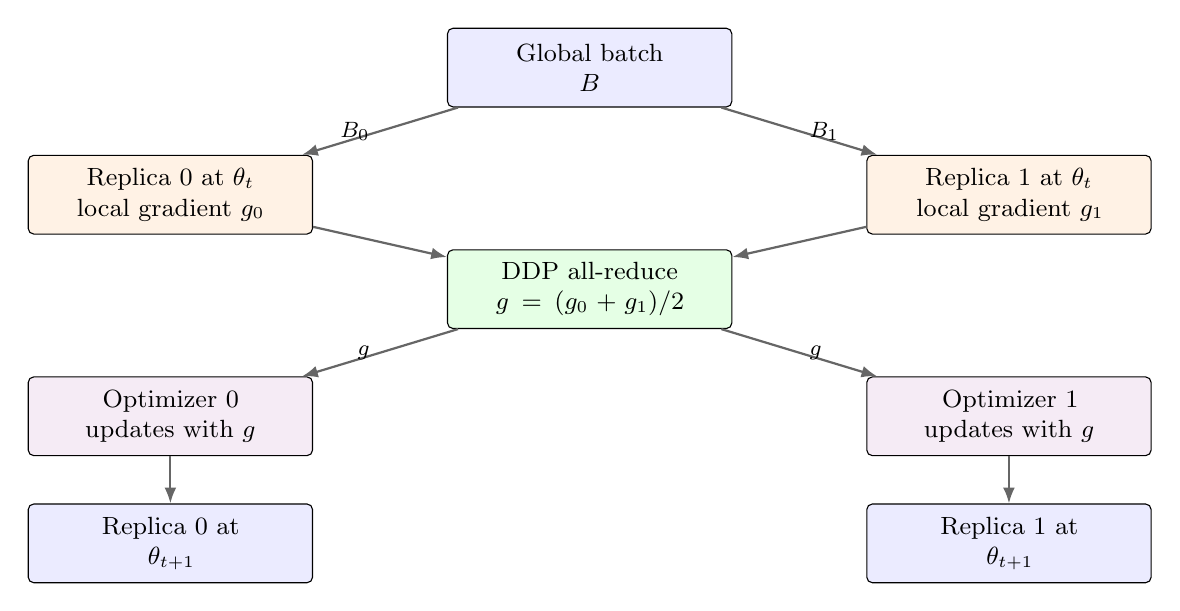
\begin{tikzpicture}[
    node distance=6mm and 17mm,
    box/.style={draw,rounded corners=2pt,align=center,minimum height=10mm,
        text width=34mm,font=\small,inner sep=3pt},
    arrow/.style={-{Latex[length=2mm]},thick,draw=black!60}
]
\node[box,fill=blue!8] (global) {Global batch\\$B$};
\node[box,fill=orange!10,below left=of global] (m0)
    {Replica 0 at $\theta_t$\\local gradient $g_0$};
\node[box,fill=orange!10,below right=of global] (m1)
    {Replica 1 at $\theta_t$\\local gradient $g_1$};
\node[box,fill=green!10,below=18mm of global] (reduce)
    {DDP all-reduce\\$g=(g_0+g_1)/2$};
\node[box,fill=violet!8,below left=of reduce] (step0)
    {Optimizer 0\\updates with $g$};
\node[box,fill=violet!8,below right=of reduce] (step1)
    {Optimizer 1\\updates with $g$};
\node[box,fill=blue!8,below=of step0] (new0)
    {Replica 0 at\\$\theta_{t+1}$};
\node[box,fill=blue!8,below=of step1] (new1)
    {Replica 1 at\\$\theta_{t+1}$};
\draw[arrow] (global) -- node[left,font=\footnotesize] {$B_0$} (m0);
\draw[arrow] (global) -- node[right,font=\footnotesize] {$B_1$} (m1);
\draw[arrow] (m0) -- (reduce);
\draw[arrow] (m1) -- (reduce);
\draw[arrow] (reduce) -- node[left,font=\footnotesize] {$g$} (step0);
\draw[arrow] (reduce) -- node[right,font=\footnotesize] {$g$} (step1);
\draw[arrow] (step0) -- (new0);
\draw[arrow] (step1) -- (new1);
\end{tikzpicture}
\caption{Each rank computes a local gradient. DDP returns the same averaged
gradient to both ranks, and each rank updates its own replica.}
\label{fig:ddp-workflow}
\end{figure}

\noindent\begin{minipage}{\textwidth}
The core PyTorch implementation uses DDP together with a distributed
sampler~\cite{pytorch-ddp,pytorch-distributed-sampler}:

\begin{lstlisting}[basicstyle=\ttfamily\footnotesize]
import os
import torch
import torch.distributed as dist
from torch.nn.parallel import DistributedDataParallel as DDP
from torch.utils.data import DataLoader, DistributedSampler

# Join the processes started by torchrun. NCCL handles GPU collectives.
dist.init_process_group(backend="nccl")

# torchrun assigns this process one GPU index on the current machine.
local_rank = int(os.environ["LOCAL_RANK"])

# Make that GPU the default CUDA device for this process.
torch.cuda.set_device(local_rank)

# Give every rank the same number of examples. If the dataset size is not
# divisible by the number of ranks, drop the tail instead of padding the
# index list with duplicate examples.
sampler = DistributedSampler(dataset, shuffle=True, drop_last=True)
loader = DataLoader(dataset, batch_size=local_batch_size,
                    sampler=sampler)

model = Model().to(local_rank)
model = DDP(model, device_ids=[local_rank])
optimizer = torch.optim.AdamW(model.parameters(), lr=learning_rate)

for epoch in range(num_epochs):
    # The rank slices differ but come from the same epoch shuffle.
    sampler.set_epoch(epoch)
    for x, y in loader:
        x = x.to(local_rank)
        y = y.to(local_rank)
        optimizer.zero_grad()
        loss = model(x, y)
        loss.backward()       # DDP synchronizes gradients here.
        optimizer.step()

dist.destroy_process_group()
\end{lstlisting}
\end{minipage}

\texttt{torchrun} starts this program once per GPU and supplies
\texttt{LOCAL\_RANK}. \texttt{DistributedSampler} partitions dataset indices
among ranks. DDP registers the gradient synchronization used by
\texttt{loss.backward()}. NanoGPT uses the same one-process-per-GPU DDP
structure~\cite{karpathy-nanogpt}. Instead of a distributed sampler, each rank
calls \texttt{get\_batch()}. A rank-dependent seed gives the ranks different
random streams.

\newpage
\section{OLMo data organization under DDP}

DDP synchronizes gradients, but it does not decide which data a rank receives.
OLMo presents training data through an indexed \texttt{InstanceSource}. An
instance index \(i\) is the address of one model input, not a token ID. The
meaning of that address depends on the concrete source. For a
\texttt{ConcatAndChunkInstanceSource} with sequence length \(S\),

\[
i \longmapsto \texttt{source[i]}
= \text{tokens}[iS:(i+1)S].
\]

Adjacent indices in this source address adjacent, non-overlapping token
ranges~\cite{olmo-concat-and-chunk-source}. This is not guaranteed for every
source. A \texttt{SamplingInstanceSource} can deliberately map multiple
indices to the same child instance when it repeats a dataset
\cite{olmo-sampling-instance-source}.

A \texttt{PackingInstanceSource} precomputes which documents belong to each
instance. When \texttt{source[i]} is called, it reads those document token
ranges, concatenates them, and pads the result to length \(S\). The loader
sees the same indexed interface even though the sources construct an instance
differently~\cite{olmo-instance-source,olmo-packing-source}.

\subsection{One index array defines the training order}

Suppose the source contains ten instances. With four instances per global
batch, OLMo retains eight shuffled indices for two complete batches and drops
the two-index tail. Suppose the retained order is

\[
[7,2,9,0,\;5,1,8,3].
\]

With four instances per global batch, reshaping the array gives one row per
optimizer step:

\[
\begin{array}{c|c}
\text{step 0} & [7,2,9,0] \\
\text{step 1} & [5,1,8,3]
\end{array}
\]

With two DDP ranks, each rank takes every second column:

\[
\begin{array}{c|cc}
 & \text{rank 0} & \text{rank 1} \\
\hline
\text{step 0} & [7,9] & [2,0] \\
\text{step 1} & [5,8] & [1,3]
\end{array}
\]

Figure~\ref{fig:olmo-index-workflow} shows the same operation as a workflow.

\begin{figure}[ht]
\centering
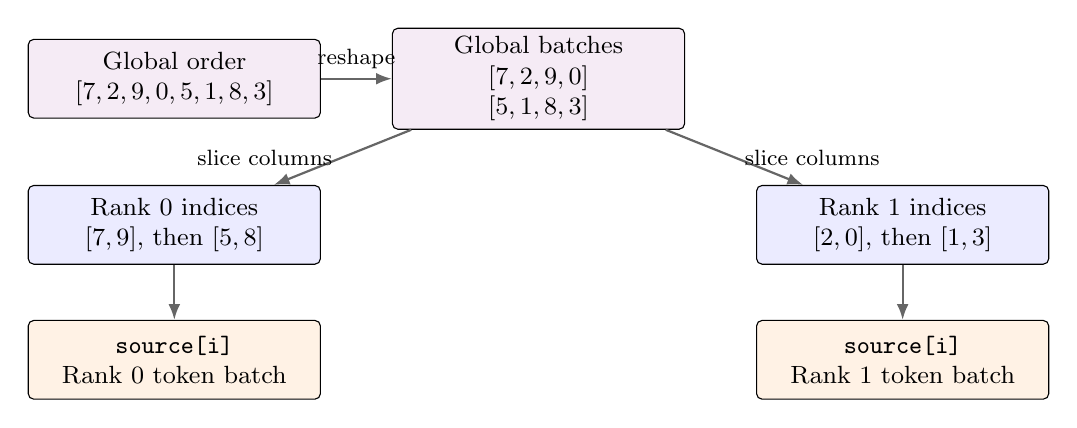
\begin{tikzpicture}[
    node distance=7mm and 9mm,
    box/.style={draw,rounded corners=2pt,align=center,minimum height=10mm,
        text width=35mm,font=\small,inner sep=3pt},
    arrow/.style={-{Latex[length=2mm]},thick,draw=black!60}
]
\node[box,fill=violet!8] (order) {Global order\\$[7,2,9,0,5,1,8,3]$};
\node[box,fill=violet!8,right=of order] (rows)
    {Global batches\\$[7,2,9,0]$\\$[5,1,8,3]$};
\node[box,fill=blue!8,below left=of rows] (r0)
    {Rank 0 indices\\$[7,9]$, then $[5,8]$};
\node[box,fill=blue!8,below right=of rows] (r1)
    {Rank 1 indices\\$[2,0]$, then $[1,3]$};
\node[box,fill=orange!10,below=of r0] (f0)
    {\texttt{source[i]}\\Rank 0 token batch};
\node[box,fill=orange!10,below=of r1] (f1)
    {\texttt{source[i]}\\Rank 1 token batch};
\draw[arrow] (order) -- node[above,font=\footnotesize] {reshape} (rows);
\draw[arrow] (rows) -- node[left,font=\footnotesize] {slice columns} (r0);
\draw[arrow] (rows) -- node[right,font=\footnotesize] {slice columns} (r1);
\draw[arrow] (r0) -- (f0);
\draw[arrow] (r1) -- (f1);
\end{tikzpicture}
\caption{OLMo decides the indices in a global batch before reading the token
sequences. Each DDP rank receives a different column slice.}
\label{fig:olmo-index-workflow}
\end{figure}

The implementation is the same transformation
\cite{olmo-composable-loader}:

\begin{lstlisting}[basicstyle=\ttfamily\footnotesize]
# One row is one global batch.
rows = global_indices.reshape(-1, instances_per_batch)

# Skip optimizer steps that were already completed.
rows = rows[batches_processed:]

# Take this DDP rank's columns from every remaining row.
local_indices = rows[:, dp_rank::dp_world_size].reshape(-1)
\end{lstlisting}

NanoGPT does not build this shared array. Each NanoGPT rank samples random
starting positions independently. Rank-specific seeds give different random
streams, but two ranks can select overlapping token windows. OLMo instead
divides each row of one shared schedule among the ranks. A scheduled index is
therefore assigned to only one rank in a global batch. With direct consecutive
chunking, different scheduled indices also mean disjoint token ranges. A
sampling source can still map different scheduled indices to the same child
instance~\cite{olmo-sampling-instance-source}.

The OLMo organization under DDP is thus:

\[
\boxed{
\texttt{source[i]}
\quad+\quad
\text{global index rows}
\quad+\quad
\text{rank column slices}
}
\]

The source determines the contents of an instance. The index rows determine
the global batches. The column slices determine the local DDP batches.

\newpage
\section{From DDP to ZeRO and FSDP}

ZeRO begins with DDP and removes one kind of replicated model state at each
stage~\cite{rajbhandari2020zero}. Let \(N\) be the number of data-parallel
ranks. Let \(P\), \(G\), and \(O\) denote the memory required by one complete
copy of the parameters, gradients, and optimizer state. These expressions
count model state only. They do not include activations or temporary
communication buffers.

\begin{center}
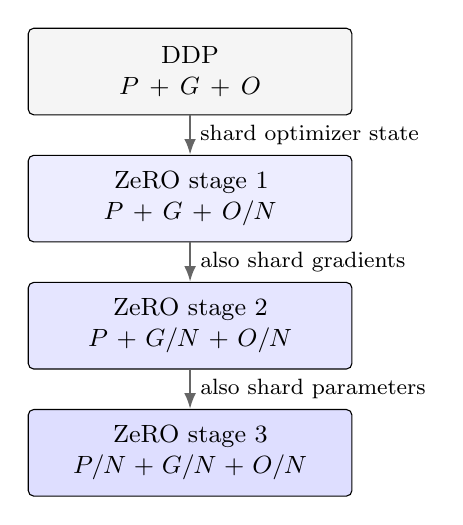
\begin{tikzpicture}[
    node distance=5mm,
    state/.style={draw,rounded corners=2pt,align=center,minimum height=11mm,
        text width=39mm,font=\small,inner sep=3pt},
    arrow/.style={-{Latex[length=2mm]},thick,draw=black!60}
]
\node[state,fill=gray!8] (ddp)
    {DDP\\\(P+G+O\)};
\node[state,fill=blue!7,below=of ddp] (z1)
    {ZeRO stage 1\\\(P+G+O/N\)};
\node[state,fill=blue!10,below=of z1] (z2)
    {ZeRO stage 2\\\(P+G/N+O/N\)};
\node[state,fill=blue!13,below=of z2] (z3)
    {ZeRO stage 3\\\(P/N+G/N+O/N\)};
\draw[arrow] (ddp) -- node[right,font=\footnotesize] {shard optimizer state} (z1);
\draw[arrow] (z1) -- node[right,font=\footnotesize] {also shard gradients} (z2);
\draw[arrow] (z2) -- node[right,font=\footnotesize] {also shard parameters} (z3);
\end{tikzpicture}
\end{center}

\subsection{ZeRO stage 1: shard the optimizer state}

For a parameter \(\theta_j\) with gradient \(g_j\), Adam performs

\[
\begin{aligned}
m_j^{(t)} &=
    \beta_1m_j^{(t-1)}+(1-\beta_1)g_j^{(t)},\\
v_j^{(t)} &=
    \beta_2v_j^{(t-1)}+(1-\beta_2)\bigl(g_j^{(t)}\bigr)^2,\\
\widehat m_j^{(t)} &= \frac{m_j^{(t)}}{1-\beta_1^t},
\qquad
\widehat v_j^{(t)} = \frac{v_j^{(t)}}{1-\beta_2^t},\\
\theta_j^{(t+1)} &=
    \theta_j^{(t)}
    -\eta\frac{\widehat m_j^{(t)}}{\sqrt{\widehat v_j^{(t)}}+\epsilon}.
\end{aligned}
\]

The optimizer state for \(\theta_j\) is \(m_j\), \(v_j\), and the step
counter \(t\). With two ranks and
\(\theta=[\theta_0,\theta_1,\theta_2,\theta_3]\), one Stage-1 update is simply

\[
\begin{aligned}
\text{rank 0: }&\quad
  \operatorname{Adam}(\theta_{0:2},g_{0:2},m_{0:2},v_{0:2})
  \longrightarrow \theta'_{0:2},\\
\text{rank 1: }&\quad
  \operatorname{Adam}(\theta_{2:4},g_{2:4},m_{2:4},v_{2:4})
  \longrightarrow \theta'_{2:4},\\
\text{all-gather: }&\quad
  \theta'=[\theta_0',\theta_1',\theta_2',\theta_3']
  \quad\text{on both ranks}.
\end{aligned}
\]

The all-gather collects the updated parameters. It does not collect the Adam
state.

\begin{lstlisting}[basicstyle=\ttfamily\footnotesize]
# ZeRO-1 update executed by every rank.
local_slice = slice(0, 2) if rank == 0 else slice(2, 4)

g_global = synchronize_gradients(g_contribution_local)
theta_local = theta[local_slice]
adam_update_(theta_local, g_global[local_slice], adam_state_local)

theta = all_gather(theta_local)
# Every rank now has [theta0', theta1', theta2', theta3'].
\end{lstlisting}

Only the optimizer state has stopped being replicated. The memory saved per
rank relative to DDP is

\[
O-\frac{O}{N}=O\left(1-\frac{1}{N}\right).
\]

Parameters and gradients remain replicated.

\subsection{ZeRO stage 2: also shard the gradients}

Stage 2 changes how the same divided update receives its gradients. A
reduce-scatter gives rank 0 only the averaged \(g_0,g_1\), and rank 1 only the
averaged \(g_2,g_3\). Each rank already has the matching Adam state, so it has
everything required for its local updates:

\[
\begin{array}{c|c}
\text{rank 0} & (g_0,g_1)+(m_0,v_0,m_1,v_1)
    \longrightarrow (\theta_0',\theta_1') \\
\text{rank 1} & (g_2,g_3)+(m_2,v_2,m_3,v_3)
    \longrightarrow (\theta_2',\theta_3')
\end{array}
\]

The ranks then all-gather \((\theta_0',\theta_1')\) and
\((\theta_2',\theta_3')\). Thus both ranks again begin the next forward pass
with the same complete \(\theta'\). Neither gradients nor optimizer state are
gathered.

\begin{lstlisting}[basicstyle=\ttfamily\footnotesize]
# Conceptual ZeRO-2 update executed by every rank.
g_local = reduce_scatter(g_contribution_local) / world
theta_local = theta[local_slice]
adam_update_(theta_local, g_local, adam_state_local)

# Rebuild the replicated model; do not gather g, m, or v.
theta = all_gather(theta_local)
\end{lstlisting}

Real implementations reduce-scatter one gradient bucket as soon as it is
ready, so they do not need to retain one complete flattened gradient. Stage 2
saves an additional

\[
G-\frac{G}{N}=G\left(1-\frac{1}{N}\right)
\]

per rank.

\subsection{ZeRO stage 3: also shard the parameters}

Stage 3 also makes the parameter ownership permanent. Rank 0 retains only
\((\theta_0,\theta_1)\); rank 1 retains only
\((\theta_2,\theta_3)\). After backward, the update is still

\[
\begin{array}{c|c}
\text{rank 0} & (\theta_0,\theta_1),(g_0,g_1),(m_0,v_0,m_1,v_1)
    \longrightarrow (\theta_0',\theta_1') \\
\text{rank 1} & (\theta_2,\theta_3),(g_2,g_3),(m_2,v_2,m_3,v_3)
    \longrightarrow (\theta_2',\theta_3').
\end{array}
\]

This time there is no all-gather at the end of the optimizer step. The new
model exists as the distributed concatenation
\(\theta'=[\theta_0',\theta_1']\mathbin{\|}[\theta_2',\theta_3']\).
When a layer is about to run, its parameter shards are temporarily
all-gathered; after that layer's computation, the temporary complete layer is
discarded.

\begin{lstlisting}[basicstyle=\ttfamily\footnotesize]
# A layer is materialized only while that layer computes.
full_layer = all_gather(theta_local)
output = forward_layer(input, full_layer)
del full_layer

# Backward returns only the gradient owned by this rank.
full_layer = all_gather(theta_local)
g_local = reduce_scatter(backward_layer(full_layer)) / world
del full_layer

# Update only the persistent local parameter shard.
adam_update_(theta_local, g_local, adam_state_local)
# No full parameter model is assembled here.
\end{lstlisting}

Stage 3 saves an additional

\[
P-\frac{P}{N}=P\left(1-\frac{1}{N}\right)
\]

per rank between computations. At this point parameters, gradients, and
optimizer state are all sharded.

Fully Sharded Data Parallel (FSDP) is PyTorch's implementation of this
stage-3 pattern~\cite{zhao2023fsdp}. In OLMo, the process mesh and sharding
policy configure PyTorch FSDP, which supplies the parameter all-gather and
gradient reduce-scatter.

\begin{center}
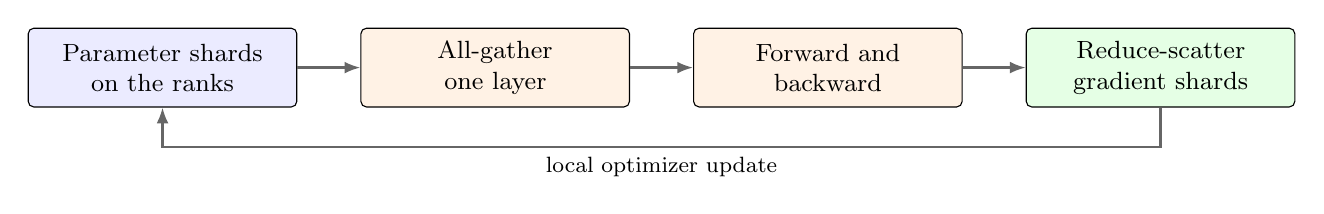
\begin{tikzpicture}[
    node distance=6mm and 8mm,
    box/.style={draw,rounded corners=2pt,align=center,minimum height=10mm,
        text width=32mm,font=\small,inner sep=3pt},
    arrow/.style={-{Latex[length=2mm]},thick,draw=black!60}
]
\node[box,fill=blue!8] (shards) {Parameter shards\\on the ranks};
\node[box,fill=orange!10,right=of shards] (gather)
    {All-gather\\one layer};
\node[box,fill=orange!10,right=of gather] (compute)
    {Forward and\\backward};
\node[box,fill=green!10,right=of compute] (reduce)
    {Reduce-scatter\\gradient shards};
\draw[arrow] (shards) -- (gather);
\draw[arrow] (gather) -- (compute);
\draw[arrow] (compute) -- (reduce);
\draw[arrow] (reduce.south) -- ++(0,-5mm) -| node[below,pos=0.25,font=\footnotesize]
    {local optimizer update} (shards.south);
\end{tikzpicture}
\end{center}

The available data-parallel modes are \texttt{ddp}, \texttt{fsdp}, and
\texttt{hsdp}~\cite{olmo-data-parallel}. The \texttt{fsdp} mode is the fully
sharded endpoint; stages 1 and 2 above explain the progression to it.

The corresponding OLMo control flow is visible in these abridged excerpts
\cite{olmo-transformer-train-module}:

\begin{lstlisting}[basicstyle=\ttfamily\footnotesize]
from torch.distributed.fsdp import FSDPModule
from torch.nn.parallel import DistributedDataParallel as DDP

# Construct the process mesh and parallelize the model.
self.world_mesh = build_world_mesh(dp=dp_config, ...)
self.model = parallelize_model(
    model,
    world_mesh=self.world_mesh,
    ...,
    dp_config=dp_config,
)

# The optimizer is built after DDP or FSDP has been applied.
self.optim = optim.build(self.model, strict=True)

# PyTorch DDP or FSDP performs its communication through autograd.
loss.backward()
self.optim.step()
\end{lstlisting}

The model is sharded before the optimizer is constructed. The optimizer
therefore receives local parameter shards and creates its per-parameter state
for those shards. Supported optimizers can be selected through configuration.
A new optimizer requires a configuration and build implementation. Ordinary
per-parameter state works with the same FSDP algorithm; global
cross-parameter state or custom communication requires additional integration.

The data assignment from Section 3 is unchanged. FSDP changes the ownership
and communication of model state, not the sequence indices assigned to ranks.
\begin{thebibliography}{99}

\bibitem{li2020pytorchdistributed}
Shen Li, Yanli Zhao, Rohan Varma, Omkar Salpekar, Pieter Noordhuis,
Teng Li, Adam Paszke, Jeff Smith, Brian Vaughan, Pritam Damania, and
Soumith Chintala.
\newblock PyTorch Distributed: Experiences on Accelerating Data Parallel
Training.
\newblock \emph{Proceedings of the VLDB Endowment}, 13(12), 2020.
\newblock \url{https://www.vldb.org/pvldb/vol13/p3005-li.pdf}.

\bibitem{pytorch-ddp}
PyTorch contributors.
\newblock Distributed Data Parallel implementation.
\newblock \url{https://github.com/pytorch/pytorch/blob/main/torch/nn/parallel/distributed.py}.

\bibitem{pytorch-distributed-sampler}
PyTorch contributors.
\newblock Distributed sampler implementation.
\newblock \url{https://github.com/pytorch/pytorch/blob/main/torch/utils/data/distributed.py}.

\bibitem{karpathy-nanogpt}
Andrej Karpathy.
\newblock nanoGPT training script.
\newblock \url{https://github.com/karpathy/nanoGPT/blob/master/train.py}.

\bibitem{olmo-composable-loader}
Allen Institute for AI.
\newblock OLMo-core composable data loader.
\newblock \href{https://github.com/allenai/OLMo-core/blob/92870a33c3fee060d57c3faec52b0b369ece85a6/src/olmo_core/data/composable/data_loader.py}{GitHub source}.

\bibitem{olmo-instance-source}
Allen Institute for AI.
\newblock OLMo-core instance-source interface.
\newblock \href{https://github.com/allenai/OLMo-core/blob/92870a33c3fee060d57c3faec52b0b369ece85a6/src/olmo_core/data/composable/instance_source.py}{GitHub source}.

\bibitem{olmo-concat-and-chunk-source}
Allen Institute for AI.
\newblock OLMo-core consecutive chunk instance source.
\newblock \href{https://github.com/allenai/OLMo-core/blob/92870a33c3fee060d57c3faec52b0b369ece85a6/src/olmo_core/data/composable/concat_and_chunk_instance_source.py}{GitHub source}.

\bibitem{olmo-packing-source}
Allen Institute for AI.
\newblock OLMo-core packing instance source.
\newblock \href{https://github.com/allenai/OLMo-core/blob/92870a33c3fee060d57c3faec52b0b369ece85a6/src/olmo_core/data/composable/packing_instance_source.py}{GitHub source}.

\bibitem{olmo-sampling-instance-source}
Allen Institute for AI.
\newblock OLMo-core sampling instance source.
\newblock \href{https://github.com/allenai/OLMo-core/blob/92870a33c3fee060d57c3faec52b0b369ece85a6/src/olmo_core/data/composable/sampling_instance_source.py}{GitHub source}.

\bibitem{rajbhandari2020zero}
Samyam Rajbhandari, Jeff Rasley, Olatunji Ruwase, and Yuxiong He.
\newblock ZeRO: Memory Optimizations Toward Training Trillion Parameter
Models.
\newblock In \emph{SC20: International Conference for High Performance
Computing, Networking, Storage and Analysis}, 2020.
\newblock \url{https://arxiv.org/abs/1910.02054}.

\bibitem{zhao2023fsdp}
Yanli Zhao, Andrew Gu, Rohan Varma, Liang Luo, Chien-Chin Huang, Min Xu,
Less Wright, Hamid Shojanazeri, Myle Ott, Sam Shleifer, Alban Desmaison,
Can Balioglu, Pritam Damania, Bernard Nguyen, Geeta Chauhan, Yuchen Hao,
Ajit Mathews, and Shen Li.
\newblock PyTorch FSDP: Experiences on Scaling Fully Sharded Data Parallel.
\newblock \emph{Proceedings of the VLDB Endowment}, 16(12), 2023.
\newblock \url{https://arxiv.org/abs/2304.11277}.

\bibitem{olmo-data-parallel}
Allen Institute for AI.
\newblock OLMo-core data-parallel configuration.
\newblock \href{https://github.com/allenai/OLMo-core/blob/92870a33c3fee060d57c3faec52b0b369ece85a6/src/olmo_core/distributed/parallel/data_parallel.py}{GitHub source}.

\bibitem{olmo-transformer-train-module}
Allen Institute for AI.
\newblock OLMo-core transformer training module.
\newblock \href{https://github.com/allenai/OLMo-core/blob/92870a33c3fee060d57c3faec52b0b369ece85a6/src/olmo_core/train/train_module/transformer/train_module.py}{GitHub source}.

\end{thebibliography}

\end{document}
